\newpage
\section{Durchführung}
\label{sec:Durchführung}

\FloatBarrier
\subsection{(a) Erzeugen einer amplitudenmodulierten Schwingung mit
Hilfe eines Ringmodulators(keine Trägerabstrahlung)}
\label{subsec:durchfuehrung_a}
Zur Amplitudenmodulation durch einen Ringmodulator wir ein Aufbau,
entsprechend des Schaltbildes in Abbildung \ref{fig:schaltung_a}, verwendet.
Anschließend wird ein Bild, das Modulationssignal sowie moduliertes
Signal im Zeitraum zeigt, am Oszillographen aufgenommen.

\begin{figure}
  \centering
  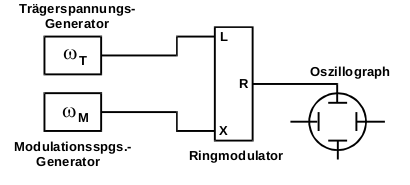
\includegraphics[width=0.7\textwidth]{figures/a_d.png}
  \caption{Verwendete Schaltung zur Amplitudenmodulation mit Ringmodulator.\cite{sample}}
  \label{fig:schaltung_a}
\end{figure}

\FloatBarrier
\subsection{(b) Untersuchung des Frequenzspektrums einer
amplitudenmodulierten Schwingung}
\label{subsec:durchfuehrung_b}
Um das Frequenzspektrum des in Abschnitt \ref{subsec:durchfuehrung_a} generierten
amplitudenmodulierten Signals zu untersuchen, wird in Abbildung
\ref{fig:schaltung_a} der Oszillograph durch einen Frequenzanalysator ersetzt.
Es wird ein Bild des Frequenzspektrums zwischen $\SI{324}{\hertz}$ und $\SI{1424}{\hertz}$
aufgenommen.

\FloatBarrier
\subsection{(c) Erzeugen einer amplitudenmodulierten Schwingung
mit Hilfe einer Gleichrichterdiode (inklusive Trägerabstrahlung)}
\label{subsec:durchfuehrung_c}
Mit Hilfe der in Abbildung \ref{fig:schaltung_c} gezeigten Schaltung,
wird ein amplitudenmoduliertes Signal mit Trägerfrequenzabstrahlung erzeugt.
Das generierte Signal wird sowohl im Zeitbereich am Oszilloskop, als auch
im Frequenzbereich am Frequenzanalysator, dargestellt.

\begin{figure}
  \centering
  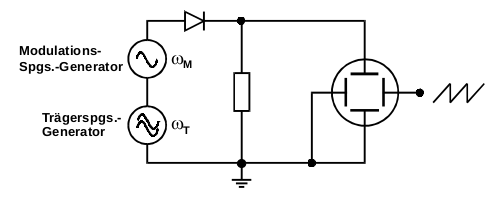
\includegraphics[width=0.7\textwidth]{figures/c_d.png}
  \caption{Verwendete Schaltung zur Amplitudenmodulation mit Diode.\cite{sample}}
  \label{fig:schaltung_c}
\end{figure}


\FloatBarrier
\subsection{(d) Erzeugen einer frequenzmodulierten Schwingung}
\label{subsec:durchfuehrung_d}
Um ein frequenzmoduliertes Signal zu generieren wird die in Abbildung
\ref{fig:frequenzmodulation} skizzierte Schaltung verwendet.
Das frequenzmodulierte Signal wird sowohl im Zeitbereich, als auch
im Frequenzbereich dargestellt.


\FloatBarrier
\subsection{(e) Untersuchung der Phasenabhängigkeit eines
phasenempfindlichen Gleichrichters}
\label{subsec:durchfuehrung_e}
Um die Phasenempfindlichkeit eines Gleichrichters zu zeigen,
wird eine Schaltung gemäß Abbildung \ref{fig:schaltung_e} verwendet.
Es werden zu eingestellten Frequenzen Spannungswerte gemessen.

\begin{figure}
  \centering
  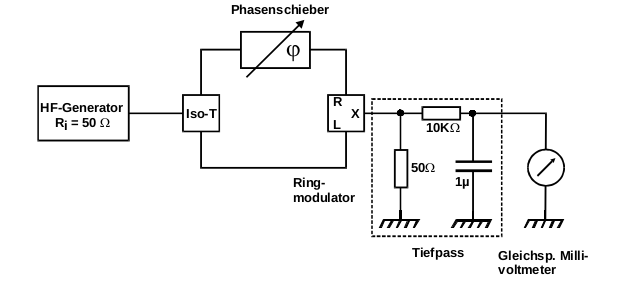
\includegraphics[width=0.7\textwidth]{figures/e_d.png}
  \caption{Verwendete Schaltung zur Untesuchung eines phasenempfindlichen Gleichrichters.\cite{sample}}
  \label{fig:schaltung_e}
\end{figure}


\FloatBarrier
\subsection{(f) Demodulation einer amplitudenmodulierten Schwingung
mit Hilfe eines Ringmodulators}
\label{subsec:durchfuehrung_f}
Um die Demodulation eines amplitudenmodulierten Signals zu veranschaulichen,
wird eine Schaltung, wie in Abbildung \ref{fig:demodulatorschaltung},
verwendet. Es werden sowohl das ursprüngliche Signal als auch das
demodulierte Signal im Zeitbereich dargestellt, sodass verglichen werden kann.


\FloatBarrier
\subsection{(g) Demodulation einer amplitudenmodulierten Schwingung
mit Hilfe einer Gleichrichterdiode}
\label{subsec:durchfuehrung_g}
Zur Veranschaulichung der Demodulation eines amplitudenmodulierten Signals
mit Hilfe von Gleichrichterdiode und Tiefpass, wird die in Abbildung
\ref{fig:gleichrichterdiode} skizzierte Schaltung verwendet.
Das Signal wird sowohl am Punkt \textbf{A} als auch nach durchlaufen des Tiefpasses
im Zeitbereich dargestellt.


\FloatBarrier
\subsection{(h) Demodulation einer frequenzmodulierten Schwingung
mit Hilfe eines Flankendemodulators}
\label{subsec:durchfuehrung_h}
Zur Demodulation eines frequenzmodulierten Signals wird die in Abbildung
\ref{fig:flankenmodulator} dargestellte Schaltung eines Flankendemodulators verwendet.
Um zu zeigen, dass das frequenzmodulierte Signal zunächst in ein
amplitudenmoduliertes umgewandelt wird, wird zunächst das Ausgangssignal
am LC-Kreis am Oszillographen dargestellt. Anschließend wird
auch das demodulierte Signal im Zeitbereich aufgenommen.
